% Research manuscript. Compile with latexmk -pdf manuscript.tex.
\documentclass[pdflatex,iicol,sn-mathphys-num]{sn-jnl}
\usepackage{amsmath,amssymb,amsthm,booktabs,tabularx,xurl,graphicx}
\newtheorem{proposition}{Proposition}
\emergencystretch=2em
\raggedbottom
\begin{document}
\title[Report-bound verification for vehicular crowdsensing]{Privacy-Preserving Report-Bound Spatiotemporal Verification for Vehicular Crowdsensing}
\author[1]{\fnm{Lili} \sur{He}}
\author[1]{\fnm{Sheng} \sur{Jiang}}
\author[1]{\fnm{Shuang} \sur{Chen}}
\author*[1]{\fnm{Lei} \sur{Zhang}}\email{8213662@163.com}
\affil[1]{\orgdiv{College of Information and Electronic Technology}, \orgname{Jiamusi University}, \orgaddress{\city{Jiamusi}, \postcode{154007}, \country{China}}}
\abstract{Vehicular crowdsensing tasks may require that an accepted report be associated with an authorised participant and an issuer-asserted event within a specified spatial and temporal policy. Verifying these conditions can disclose sensitive movement information, while independently valid credentials, event attestations and report data do not by themselves establish that they refer to the same submission. This paper presents a report-bound zero-knowledge verification relation linking an authority-issued credential, a certified event issuer, private event coordinates, a task-specific tag, and a context derived from the task, challenge and submitted report envelope. The gateway reconstructs the public context from its own task configuration and the received bytes, verifies the proof, and applies a task-scoped duplicate-acceptance rule. A prototype combines Groth16 proofs with in-circuit EdDSA signature verification, Merkle membership for discrete regions, an ML-KEM-based encrypted report envelope, an optional credential-linked identity ciphertext for authorized opening, and a private active-credential membership check. On an Apple M1, the complete in-process workflow with the active-set circuit averages 410.47 ms over 30 runs, and its serialized proof occupies 164 bytes. A controlled receipt-transfer ablation illustrates the effect of holder binding, and gateway tests exercise report substitution and task-scoped duplicate acceptance. The event issuer's observation procedure and credential enrolment are explicit trust assumptions.} 
\keywords{Vehicular crowdsensing, zero-knowledge proof, report authentication, spatiotemporal policy, privacy, duplicate detection}
\maketitle

\section{Introduction}
Vehicular crowdsensing uses observations collected by participating vehicles to support applications such as road monitoring and urban sensing. A task can require a report to originate from a designated region during a given interval. Verifying those conditions while preserving privacy calls for more than concealing a vehicle identifier: a precise location and time may themselves expose a participant's movements. Privacy-preserving crowdsensing research has therefore examined anonymous participation, protected reports and duplicate detection~\citep{Ni2020SPOON,Xu2021TaskMatching}.

This paper considers a gateway deciding whether to accept one report for one task. The gateway needs a verifiable connection among a participant's authorisation, an event issuer's assertion, the applicable task policy, and the bytes submitted as the report. If these checks are performed on independently selected evidence, successful checks alone do not show that all components concern the same submission. We address this coordination problem through a zero-knowledge relation whose private witness contains the credential, certified event issuer, receipt and event coordinates. The public statement includes a task-scoped tag and a context derived from the configured task, challenge and received report envelope.

The gateway checks the proof and records the tag to reject a repeated contribution with the same credential in the same task. It reconstructs the task and report context itself, rather than accepting those values as free configuration supplied by the participant. The resulting decision is per credential and depends on the enrolment policy when interpreted as a limit per person or vehicle. An event signature authenticates an issuer's assertion, and its physical meaning depends on the issuer's observation procedure. It does not establish the truth of the sensor value by itself.

The construction is complementary to TST-Audit~\citep{He2026TSTAudit}, which addresses verification of accumulated spatiotemporal coverage. TST-Audit defines an abstract microproof interface with a hidden location and time, a public grid and epoch, a credential-based scoped nullifier, and an assigned edge context. Here the verification object is a task report and the proposed relation explicitly connects an issuer-signed event to the bytes submitted for that report. This difference in object and relation does not imply that every instantiation of TST-Audit's abstract interface lacks report binding.

This paper makes three contributions. First, it specifies a report acceptance relation in which the same participant secret links the credential, issuer receipt and task-scoped tag. Second, it describes executable instantiations with private issuer authorisation, explicit context reconstruction, integer spacetime bounds, discrete-region membership and credential-linked identity encryption. Third, it evaluates an implemented proof and gateway with substitution and replay tests, a controlled receipt-transfer ablation, and separate proof-generation and verification measurements.

\section{Related Work}
\paragraph{Private crowdsensing and duplicate detection.} Ni et al. combine anonymous credentials, encrypted reports and duplicate-report detection in SPOON~\citep{Ni2020SPOON}. Xu et al. study private task matching and multiple-submission detection with a per-task submission rule~\citep{Xu2021TaskMatching}. Zhu et al. use privacy-preserving hybrid sensing and duplicate detection in smart parking~\citep{Zhu2022HybridSensing}. Anonymous reporting and task-scoped duplicate control are consequently established research directions. The construction examined here concerns a particular jointly verified relation among the report bytes, an authorised event issuer, a credential and a task policy.

\paragraph{Spatiotemporal evidence and coverage.} TST-Audit~\citep{He2026TSTAudit} specifies per-record microproofs and uses authenticated aggregate state for regional coverage auditing. Its published microproof interface associates a hidden event with a public grid and epoch and includes credential-based uniqueness in that scope. The task-level report relation studied here has a different acceptance object; neither work's interface should be treated as a complete substitute for all possible instantiations of the other.

Location-proof work addresses independent witnesses, distance constraints and time consistency~\citep{Brito2025DecentralizedPoL}. Brito et al. also consider content provenance with multiple observers of physical events~\citep{Brito2026ContentProvenance}. Bogdanov et al. use trusted-device-signed locations for privacy-preserving vehicle-policy proofs~\citep{Bogdanov2025VehiclePolicy}; Ernstberger et al. study zero-knowledge location properties using floating-point arithmetic~\citep{Ernstberger2025ZKLP}. These studies demonstrate that location evidence, privacy and content provenance have substantial prior art; the distinctions considered here are the report-specific relation and its implementation and evaluation, under its stated trust model.

\paragraph{Verifiable encryption.} Verifiable encryption has long been studied for applications such as escrow~\citep{CamenischShoup2003}. We apply a credential-linked identity ciphertext to the report relation; the underlying encryption and proof techniques are established primitives.

\paragraph{Data authenticity.} IoT Notary examines attestable sensor capture and logging~\citep{Panwar2022IoTNotary}, while BlockSense studies trustworthy crowdsensing and data quality~\citep{Huang2024BlockSense}. These systems address aspects of data origin and quality that are separate from mathematical verification of the policy relation in this paper.

Table~\ref{tab:comparison-context} compares the verification objects and explicitly described mechanisms of the closest studies. In particular, SPOON already combines anonymous reporting and double-report identification, while TST-Audit already specifies a credential-linked, grid--epoch-scoped microproof. Thus, anonymity or a scoped tag alone is not a distinguishing contribution here. Bogdanov et al. already use signed location claims in privacy-preserving vehicle-policy verification, and Brito et al. examine content provenance using independent witnesses. The contribution evaluated in this paper is the specific report-acceptance relation that ties a credential secret, an issuer-signed event and the received report envelope to a task-scoped tag, together with its executable extensions and controlled substitution tests. This characterization does not imply that an alternative instantiation of an earlier interface cannot provide a similar relation.

\begin{table*}[t]
\centering\small
\caption{Comparison of the reported research objects and mechanisms. Entries summarize the cited descriptions; they do not assert that an unlisted feature is absent.}\label{tab:comparison-context}
\begin{tabularx}{\textwidth}{@{}p{.14\textwidth}p{.22\textwidth}p{.29\textwidth}X@{}}
\toprule
Work & Main verification or service object & Explicit mechanisms in the cited work & Relation to the focus of this paper \\\midrule
SPOON~\citep{Ni2020SPOON} & Private task allocation and selection of mobile sensing reports & Location- and credit-based recruitment; anonymous credentials; encrypted reporting; identification of users submitting multiple reports for a task in a reporting period & The present evaluation targets a specified receipt--holder--envelope relation for one task report, rather than task recruitment or credit-based selection. \\
TST-Audit~\citep{He2026TSTAudit} & Auditable aggregate grid--epoch coverage & A pluggable microproof for hidden event location and time, credential validity and grid--epoch uniqueness; folding and Merkle-sum-tree coverage commitments & The present acceptance object is an individual task report with an explicit signed event and submitted-envelope binding; TST-Audit's interface permits different concrete microproof instantiations. \\
Bogdanov et al.~\citep{Bogdanov2025VehiclePolicy} & Vehicle travel compliance for subsidies and taxation & A trusted witness device signs location claims; zero-knowledge computations check trajectory-dependent geographic conditions & The present relation checks one issuer-asserted event and report with a task-scoped acceptance tag, instead of computing a distance or territorial fraction over a trajectory. \\
Brito et al.~\citep{Brito2026ContentProvenance} & Physical-event and content-provenance evidence & A witnessing zone combines distance bounds, independent witness decisions, commitments and a quorum-signed evidence object & The present prototype evaluates a single certified issuer's assertion and a private report-acceptance relation under its issuer-trust assumption; witness quorum and contextual sensing are the cited work's emphasis. \\
This paper & Acceptance of an individual task report & One proof links the credential, issuer receipt, task tag and received envelope; optional region, identity-encryption and active-set checks are implemented & The evaluation isolates receipt transfer in a controlled ablation and measures proof operations for four implemented relations. \\
\bottomrule
\end{tabularx}
\end{table*}

\begin{figure*}[t]
\centering\includegraphics[width=.94\textwidth]{architecture.pdf}
\caption{Conceptual report verification workflow. The authority certifies participants and issuers; the gateway reconstructs the context and checks the proof. The recipient authenticates and decrypts the verified envelope. In the tested gateway, these roles are colocated and authentication precedes acceptance.}\label{fig:architecture}
\end{figure*}

\section{System Model and Problem Formulation}
\label{sec:model}

We consider a vehicular crowdsensing task in which each accepted report must be associated with an authorised participant and a spatiotemporal event satisfying the task policy. The decision is made for an individual submitted report. A registration authority issues participant credentials and authorises event-evidence issuers. A participant prepares a report, obtains an issuer-signed event receipt, and constructs a zero-knowledge proof. A gateway verifies the proof and maintains task-specific acceptance state. The gateway obtains task parameters and the authority's public key from authenticated configuration. Figure~\ref{fig:architecture} illustrates the roles and evidence flow.

For a task identifier $\mathsf{id}$, let the policy $P=(\boldsymbol{\ell},\boldsymbol{u})$ be an axis-aligned box over integer coordinates $(x,y,t)$. An event is eligible when $\ell_j\leq z_j\leq u_j$ for each coordinate of $\boldsymbol z=(x,y,t)$. The representation and physical meaning of the coordinates are fixed by the application. The prototype uses unsigned 32-bit coordinates and inclusive bounds; the first two coordinates are planar grid coordinates and the third is a time value. A second circuit additionally requires $(x,y)$ to belong to an authorised finite set of grid cells committed by a Merkle root. The verifier configuration is assumed to assign each task identifier to one immutable box and, for this variant, one root; the prototype snapshots that configuration.

The authority is trusted to enrol authorised participants and issuers and to protect its signing key. An authorised event issuer is assumed to follow the observation procedure used to assign the signed event coordinates. Participants and the communication network may be adversarial: an attacker may substitute reports or receipts, attempt to change task parameters, submit a proof under a different credential, or replay an earlier submission. The gateway is trusted to use the configured task and authority, a trustworthy clock, and its acceptance state. An issuer's signature authenticates its event assertion and associated report context; the physical accuracy of that assertion depends on the issuer's observation procedure.

The intended acceptance condition is: (i) an enrolled participant secret and an authorised issuer support the same receipt; (ii) the signed event satisfies the configured policy; (iii) the receipt refers to the current task, challenge and submitted report bytes; and (iv) the participant secret has not already been used to produce an accepted report for this task. Condition~(iv) is per credential. Its interpretation as a per-person or per-vehicle rule additionally depends on the enrolment policy and on participants not sharing their secrets.

\section{Report-Bound Spatiotemporal Proof}
\label{sec:protocol}

\subsection{Public context and credentials}
\label{sec:context}

Let $\mathbb F$ denote the circuit field, and let $H$ be the field hash used by the circuit. Domain labels distinguish hashes with different purposes. For clarity, let $H_d(v_1,\ldots,v_k)=H(d,v_1,\ldots,v_k)$. The authority has public verification key $A$. A participant selects a nonzero secret $s$ from a high-entropy distribution and receives an authority signature $\sigma_A$ on $H_{101}(s)$. An event issuer has a verification key $W=(W_x,W_y)$ and an authority signature $\sigma_W$ on $H_{102}(W_x,W_y)$. The participant secret, both signatures and the issuer key are private witnesses in the proof. Issuance itself is not a blind-issuance protocol in the prototype.

The gateway issues a fresh challenge $q=(n,e)$ containing a random nonce $n$ and expiry time $e$. The participant encapsulates a fresh key to the authenticated recipient using ML-KEM-768~\citep{NIST2024MLKEM}, derives an AES-256-GCM key with HKDF-SHA-256, and encrypts the sensed report into an envelope $R$ containing the KEM ciphertext and authenticated ciphertext. For task record $T=(\mathsf{id},\boldsymbol{\ell},\boldsymbol u)$ and submitted envelope $R$, both parties derive
\begin{align}
 \mathsf{tid}&=\mathsf{TaskField}(\mathsf{id}),\\
 c&=\mathsf{ContextField}(T,q,R),
\end{align}
where the prototype uses SHA-256, domain-separated task encoding, a JSON encoding of the task and challenge, and a SHA-256 digest of the exact submitted bytes; the resulting digests are reduced to field elements. The verifier reconstructs $\mathsf{tid}$ and $c$ from its own task record, its issued challenge and the bytes it receives. Hence neither a participant-selected task policy nor a participant-supplied digest is accepted as the verifier's configuration. Task identifiers must not be reused for a different policy within the same deduplication domain.

The participant computes a context-dependent holder value $h=H_{103}(s,c)$ and presents it to the issuer as part of the receipt request. Following its event-observation procedure, the issuer signs
\begin{equation}
 m=H_{104}(c,h,x,y,t), \qquad \sigma_E=\mathsf{Sign}_{W}(m).
 \label{eq:receipt}
\end{equation}
Thus the signed message contains a context-specific value derived from the participant secret as well as the event coordinates. The issuer must receive enough authenticated task and challenge information to apply its own issuance rules.

\subsection{Proof relation}
\label{sec:relation}

The public instance is $(A,\mathsf{tid},c,N,\boldsymbol{\ell},\boldsymbol u)$, where $N$ is the participant's task-scoped tag. The private witness contains $(s,\sigma_A,W,\sigma_W,\sigma_E,x,y,t)$. The proof states that these values satisfy
\begin{align}
 &s\ne 0, \quad \mathsf{Verify}_A(\sigma_A,H_{101}(s))=1,\label{eq:cred}\\
 &\mathsf{Verify}_A(\sigma_W,H_{102}(W_x,W_y))=1,\label{eq:issuer}\\
 &\mathsf{Verify}_W\!\left(\sigma_E,H_{104}(c,H_{103}(s,c),x,y,t)\right)=1,\label{eq:event}\\
 &N=H_{105}(s,\mathsf{tid}),\label{eq:nullifier}\\
 &0\leq \ell_j\leq z_j\leq u_j<2^{32},\quad j\in\{1,2,3\}.
 \label{eq:policy}
\end{align}
The encoded signing keys must satisfy the curve and subgroup requirements of the signature implementation. Equations~\eqref{eq:cred}--\eqref{eq:event} use the same participant secret and context in the credential and event checks. Equation~\eqref{eq:nullifier} uses that secret again for duplicate detection, and Eq.~\eqref{eq:policy} checks the private event against public task bounds. The circuit range-constrains both event coordinates and policy endpoints before comparison, so the arithmetic comparison represents the stated unsigned integer relation.

\subsection{Discrete region membership}
For a nonrectangular set of permitted grid cells, the configured verifier builds a fixed-depth Merkle tree and adds its root $r_{\mathrm{reg}}$ to the public statement. A valid leaf is $H_{202}(x,y)$; internal nodes are $H_{203}(\mathit{left},\mathit{right})$, and unused leaves use a separate domain label. The participant supplies a private authentication path and Boolean direction bits. The circuit recomputes the root from the same signed $(x,y)$ appearing in Eq.~\eqref{eq:event} and checks equality with $r_{\mathrm{reg}}$. The implementation uses depth eight, with up to 256 distinct authorised coordinate pairs; the policy box and time interval are still checked. The verifier obtains the root from its trusted task configuration, and the task identifier is bound to this immutable root by that configuration. The root is not part of the signed context itself. Membership therefore establishes inclusion in the configured discrete set; the mapping from physical geography to cells is an input to policy construction.

The participant submits $(N,\pi,R,n)$, where $\pi$ is a proof for the public instance. The report recipient authenticates and decrypts $R$ using the encapsulated key. In the region-gateway implementation the gateway is also the recipient: it verifies the proof and the ciphertext authentication tag before returning the plaintext. In the research prototype, the signature scheme is EdDSA on the BN254 twisted-Edwards curve, $H$ is MiMC as implemented by the selected cryptographic library, and the proof system is Groth16 over BN254. Its circuit-specific setup and verification key are generated before report verification. The resulting proof verifies the specified relation under the proof-system, hash and signature assumptions.

\subsection{Credential-linked identity encryption}
An optional accountability circuit extends the region relation with an encrypted registry identity point $I$. The registrar signs the binding $\sigma_I=\mathsf{Sign}_A(H_{301}(H_{101}(s),I_x,I_y))$ for the same secret-derived commitment used in Eq.~\eqref{eq:cred}. The auditor has a trusted public key $P_A=[a]B$ in the prime-order group generated by $B$. For a fresh secret scalar $\rho$, the participant forms $C_1=[\rho]B$ and $C_2=I+[\rho]P_A$. The proof additionally verifies the registrar's binding signature and the two encryption equations, using the same $s$ as the report credential. The identity point and $\rho$ remain private; $P_A,C_1,C_2$ are public proof inputs. The verifier pins $P_A$ and reconstructs the remaining task inputs from trusted configuration and received bytes.

An authorised auditor can compute $I=C_2-[a]C_1$ from a verified record and resolve it through the registrar's protected identity mapping. The prototype demonstrates decryption to the registered group point; authentication of the real-world registry and authorization of an opening are external procedures. The proof verifies the encryption relation and its binding to the credential. This group-based encryption is distinct from the ML-KEM report envelope.

\subsection{Active credential membership}
A further circuit extends the accountability relation with a private membership path for the credential currently in use. The registrar maintains a set of active credential commitments $D=H_{101}(s)$. Each occupied leaf is $H_{402}(D)$, nodes use $H_{403}$, and empty leaves use a separate label. The circuit derives $D$ from the same secret as the credential, receipt and task tag and recomputes the configured active-set root along an eight-level private Merkle path. The verifier selects the current root from its trusted configuration. Removing a credential changes the root; a proof generated for the earlier root does not verify against the updated root. The prototype models the sets and root snapshots in memory, with up to 256 credential slots. In the active-set gateway, policy updates and acceptance use the same lock; the instance rejects earlier versions, previously used roots and reinstatement of a credential it recorded as removed. Authenticated root distribution and protection against rollback across restarts are responsibilities of the surrounding configuration service.

\subsection{Gateway acceptance}
\label{sec:acceptance}

On submission, the gateway looks up the unconsumed challenge by nonce and checks it against its clock. It reconstructs the public statement from the configured authority, task, stored challenge, received report bytes and submitted tag. The gateway accepts only if the challenge is current, $N$ has not already been accepted for this task, and proof verification succeeds. In the region-gateway variant, successful ciphertext authentication is also required before acceptance and plaintext delivery. A successful acceptance consumes the challenge and records $N$. These state changes are performed under a single lock in the experimental gateway; failed proof verification does not consume an unexpired challenge. This state is in memory and applies to one gateway instance.

Because $N$ depends on the task identifier rather than on the challenge, changing a challenge does not by itself create a new tag for the same credential and task. The rule prevents acceptance of a second contribution with the same computed tag in that gateway state. A fresh challenge associates the receipt with the current submission but does not alone show that the underlying sensor measurement was newly captured~\cite{Birkholz2023RATS}.

\subsection{Conditional security and privacy}
\label{sec:interpretation}

\begin{proposition}[Task-scoped single acceptance]
Assume soundness of the proof relation. For a fixed task identifier and participant secret, if the gateway atomically checks and records the task tag on each successful submission, it accepts at most one report with that secret in its maintained state, except with the proof system's soundness error.
\end{proposition}
\begin{proof}
Equation~\eqref{eq:nullifier} deterministically maps the fixed secret and task identifier to the same tag for each submission, independently of the challenge. On the first successful acceptance, the gateway records that tag. Atomic checking and recording prevents a concurrent or subsequent submission carrying the same tag from creating another successful acceptance in that state.
\end{proof}


The gateway's reconstruction of $c$ and Eq.~\eqref{eq:event} connect the received byte string to the signed event. Replacing those bytes while retaining the same proof changes the reconstructed context unless the resulting field values collide. Similarly, using a copied receipt with a different secret requires satisfying the holder equality and the credential and receipt checks for that secret. These statements apply under the stated relation and trusted configuration.

The proof keeps the participant secret, credential, event coordinates and issuer key out of its public witness. The gateway still sees task parameters, challenge, tag, proof, received envelope and communication metadata. The tag is intentionally stable within a task. Any claim that tags from different tasks cannot be linked requires an appropriate keyed-hash assumption for $H_{105}(s,\cdot)$ as well as consideration of the other visible fields; it cannot be established solely by observing different tag values in a finite test. In the encrypted-report workflow, the prototype uses ML-KEM-768 key encapsulation, HKDF-SHA-256 and AES-256-GCM with a fresh randomly generated nonce, authenticating the task identifier as associated data. The proof binds the resulting ciphertext envelope, rather than the plaintext, to the event receipt. Confidentiality depends on an authenticated recipient public key, secure key management and the KEM and authenticated-encryption assumptions; envelope length and network metadata remain visible. ML-KEM protects the report key, while the EdDSA and Groth16 proof components are not post-quantum primitives. The region gateway checks ciphertext authenticity before accepting and returning the report.


\section{Evaluation}
\label{sec:evaluation}

We implemented the relation in Go using gnark 0.16.4 and gnark-crypto 0.21.1-0.20260913224755-1409fe592052. The evaluation was run on an Apple M1 computer with 16 GiB memory, macOS 27.2 and Go 1.26.8; Go reported eight logical processors. The participant, authority, issuer and gateway were represented by software objects. The event values and sensing report used below were synthetic. These measurements characterize the specified cryptographic operations on this computer.

\subsection{Functional and substitution tests}
A valid witness generated an actual Groth16 proof that the gateway verified from its reconstructed public input. The test suite changed individual coordinates, time, report context, credential secret, signatures, task tag and policy endpoints. It also tested an honestly signed event outside a policy and an event at inclusive endpoints. Each invalid case was rejected by the constraint solver; the valid boundary case passed. Additional checks rejected an authority-certified identity or order-two issuer point and an off-curve issuer or signature point.

In the gateway tests, proof verification rejected a modified encrypted report and left the live challenge available for the subsequent valid submission. An unknown or expired challenge was rejected. Two concurrently submitted valid proofs used different challenges but the same task-scoped tag: exactly one submission succeeded in the single gateway instance. The region gateway separately checked the received ML-KEM envelope and returned plaintext only after proof and authentication checks succeeded. Separate envelope tests authenticated and decrypted valid ciphertexts, while rejecting changed KEM or payload bytes, a wrong task identifier and a different recipient key. For the region circuit, two permitted cells yielded valid Groth16 proofs; proof generation rejected altered paths, directions, signed coordinates and an honestly signed cell outside the configured set, while a proof checked against a different root failed verification. For the accountability circuit, a valid proof was verified and the auditor recovered the bound identity point. Altering the auditor key or ciphertext, substituting a different identity or credential binding, and using invalid points or randomizers were rejected in the tested cases. For active membership, a proof for an enrolled credential verified against the original root and failed against the updated root after removal; a different active credential generated a valid proof against the new root. An integrated gateway test also exercised active-root updates, report decryption, identity-ciphertext evidence and task-scoped duplicate rejection in the same process. A separate concurrency test exercised both forced orderings and four synchronized races between root update and report submission. The resulting outcomes respected the single-instance ordering; a second old-root proof was rejected after the update, and Go race detection reported no data race in these cases. These tests exercise specified cases in the software model.

\subsection{Holder-binding ablation}
To isolate the holder association, we constructed a comparison circuit with the same credential, issuer-certificate, event, context, bounds and tag checks, except that the issuer's receipt contains a constant in place of $H_{103}(s,c)$. The issuer signs this modified receipt format. The comparison is an intentionally constructed ablation and is not an implementation of a published protocol.

Two participants had different valid credentials and tags but used the same task, challenge, report and event. The attacker was assumed to obtain the victim's receipt, context and event before the challenge was consumed. In the full relation, both participants' own receipts satisfied their corresponding witnesses, whereas substituting the victim's receipt into the attacker's witness failed the constraint solver. In the ablation, the substituted receipt satisfied the circuit and the attacker's resulting Groth16 proof verified. Table~\ref{tab:ablation} summarizes this case. The experiment isolates the effect of the holder field under these assumptions.

\begin{table}[t]
\centering\caption{Controlled receipt-transfer ablation.}\label{tab:ablation}
\begin{tabular}{@{}lcc@{}}\toprule
Receipt relation & Own receipt & Copied receipt \\\midrule
Holder bound & Accepted & Rejected \\
Bearer control & Accepted & Accepted \\\bottomrule
\end{tabular}\par\vspace{2pt}
\footnotesize The bound cases and the bearer own-receipt case are constraint-solver checks; the copied-receipt bearer case also has a verified Groth16 proof.
\end{table}

\subsection{Proof cost}
The rectangle circuit contains 29,833 R1CS constraints, including the three signature-verification relations and the policy checks; the depth-eight discrete-region circuit contains 35,798, the region-plus-accountability circuit contains 62,627, and the additional active-membership circuit contains 68,592. For each of the four circuits, after one warm-up, 30 proofs were generated and verified using one setup and a valid synthetic witness per run. The fixture, task and event were held constant, while the challenge and synthetic report bytes varied. Times were measured around the library's proving and verification calls; credential and receipt generation, identity-ciphertext construction and opening, credential-set updates, witness construction, report encryption, communication and gateway processing were outside those intervals. Each circuit was compiled and set up once. We report the sample mean and sample standard deviation for the repeated operations (Table~\ref{tab:cost}); individual measurements are shown in Fig.~\ref{fig:bench}. All four serialized proofs occupy 164 bytes; serialized public witnesses are 364, 396, 588 and 620 bytes for the rectangle, region, accountability and active-membership circuits, respectively. These sizes are distinct from the complete report submission.

\begin{table*}[t]
\centering\small\caption{Local Groth16 operation costs and serialized sizes.}\label{tab:cost}
\begin{tabular}{@{}lrrrr@{}}\toprule
Quantity & Rectangle & Region & Accountability & Active set \\\midrule
Constraints & 29,833 & 35,798 & 62,627 & 68,592 \\
Compilation (one run), ms & 103.84 & 50.35 & 71.96 & 76.22 \\
Setup (one run), s & 2.596 & 2.182 & 3.204 & 4.424 \\
Proving, ms (mean $\pm$ SD) & $146.74\pm10.53$ & $214.28\pm8.76$ & $303.93\pm12.02$ & $422.47\pm23.72$ \\
Verification, ms (mean $\pm$ SD) & $1.027\pm0.088$ & $0.995\pm0.058$ & $1.056\pm0.257$ & $1.016\pm0.038$ \\
Proof / public witness, bytes & 164 / 364 & 164 / 396 & 164 / 588 & 164 / 620 \\\bottomrule
\end{tabular}
\end{table*}

\begin{figure*}[t]
\centering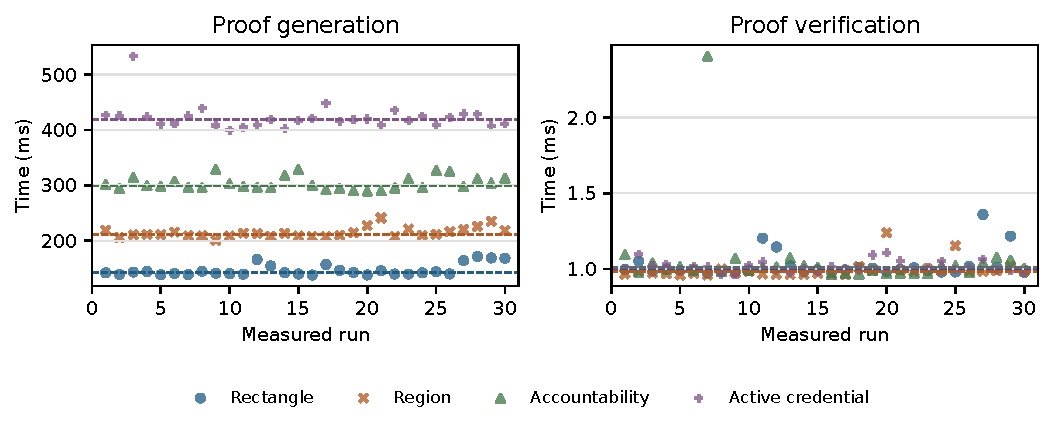
\includegraphics[width=.9\textwidth]{benchmark.pdf}
\caption{Thirty local proof-generation and verification measurements per circuit after one warm-up. Dashed lines indicate medians; setup, signing, encryption and network operations are excluded.}\label{fig:bench}
\end{figure*}

\subsection{In-process report workflow}
We separately measured the full active-credential workflow in a single process on the same computer. The experiment configured 256 region leaves and 256 active-set entries; 31 entries corresponded to generated test participants and the remaining entries were synthetic filler digests. After setup and one warm-up, 30 distinct test credentials submitted one synthetic report each under the same task. Each run included challenge issuance, ML-KEM report encryption, fixture-side signature and witness construction, proof generation and serialization, and gateway proof verification, authenticated decryption and duplicate checking. The issuer and registration operations were represented by software fixtures, and there was no network transfer or physical measurement.

The elapsed time from issuing the challenge to successful gateway acceptance was $410.47\pm17.90$ ms (mean $\pm$ sample standard deviation, $n=30$). Within this interval, proof generation averaged 408.09 ms, encryption averaged 0.036 ms, fixture signing and witness construction averaged 0.952 ms, and gateway verification, decryption and duplicate checking averaged 1.368 ms. Opening the identity ciphertext in an accepted in-memory record was timed separately and averaged 0.336 ms; this measurement excludes independent re-verification and registry lookup. Compilation, setup, enrollment, key distribution and communication were outside the timed interval.

For a 40-byte synthetic plaintext, the ciphertext envelope occupied 1,158 bytes. The encoded envelope, proof, challenge nonce, task tag and two compressed identity-ciphertext points together occupied 1,482 bytes in the measured representation. This component sum excludes transport framing and configuration distribution; the 620-byte public witness was reconstructed locally for verification rather than included in that sum.

\section{Discussion}
\label{sec:discussion}
The experiments show how holder binding changes the receipt-transfer outcome in the controlled scenario and how the policy relation can be extended from a rectangle to a discrete region, an encrypted identity point and an active credential set. These extensions retain a constant serialized Groth16 proof size in the tested implementation while increasing the circuit and public-witness sizes. The one-time setup measurements, repeated proof measurements and in-process workflow measurements describe different operations and are reported separately.

The gateway reconstructs its public inputs from trusted configuration and the received envelope, while the issuer's observation and the enrolment process supply the physical and administrative meaning of the cryptographic relation. Cross-task unlinkability and report confidentiality also depend on the stated hash, key-management and metadata assumptions.

\section{Conclusion}
This paper formulates an individual-report acceptance relation for vehicular crowdsensing. The relation joins an authorised credential, an issuer-certified spatiotemporal event, the configured task and the submitted report envelope; it also exposes a task-scoped tag for duplicate checking. A Groth16-based prototype instantiates the relation using in-circuit signatures, fixed-width policy comparisons, discrete-region proofs, optional identity encryption and active-membership checks, and externally reconstructed public context. The resulting claims are conditional on credential enrolment, issuer observation, trustworthy gateway configuration, and the stated cryptographic assumptions. The local experiments verify the stated substitution cases and quantify proof costs for this implementation; the holder-binding ablation isolates the effect of connecting an issuer receipt to the credential secret in the tested transfer scenario.

\bibliography{references}

\section*{Statements and Declarations}
\noindent\textbf{Funding:} This study received partial support from the Heilongjiang Provincial University Teacher Scientific Research Business Fee (2018-KYYWF0941), the Heilongjiang Provincial Natural Science Foundation Joint Fund Cultivation Project (PL2024F002), the National Foreign Expert Key Support Project (D2O25O185), and the Heilongjiang Provincial Undergraduate University Excellent Young Teacher Fundamental Research Support Plan (YQJH2024239).

\noindent\textbf{Competing interests:} The authors declare that they have no known competing financial interests or personal relationships that could have appeared to influence the work reported in this paper.

\noindent\textbf{Author contributions:} Lili He: supervision. Sheng Jiang: methodology, software, investigation, formal analysis. Shuang Chen: writing -- original draft. Lei Zhang: supervision, corresponding author.

\noindent\textbf{Data and code availability:} The prototype code and the experimental records supporting the findings are provided in the supplementary files accompanying this manuscript.
\end{document}
